% -*- mode:LaTex; mode:visual-line; mode:flyspell; fill-column:75-*-

\chapter{Background} \label{chap:background}

As eluded to in \ref{chap:introduction}, SLAM systems that run on real robots can be crudely divided into \emph{front-end} and \emph{back-end}. This chapter is a primer on algorithms and methods used in the \emph{front-end} and \emph{back-end}.

\section{The Front End}

The robotic paradigm describes the relationship of an agent interacting with its environment through the \emph{sense-plan-act} control loop. SLAM being in the sense paradigm, deals with processing the raw environment sensor readings to a structured representation that can be used in downstream tasks.

The front end deals with data preparation, modeling and data association such that it is amenable to the underlying optimization. More often than not, the choice of front-end is sensor dependent. For instance, many visual SLAM systems resort to feature based sparse representations, while RGB-Depth sensor based systems resort to direct methods that utilize all the pixels in the input frame. This distinction in the choice of front-end directly influences the choice of map representation in a SLAM system. In particular, a popular choice with visual SLAM system is to use an \emph{explicit} map representation as a collection of 3D points, that is \emph{triangulated} from multiple 2D image feature correspondences, while dense front-end systems, rely on surfel representations or on volumetric representations such as occupancy grids. More recently, after the seminal work \cite{newcombeKinectFusionRealtimeDense2011}, \emph{implicit} map representations have gained popularity as a candidate representation for RGB-Depth SLAM systems.

In this work, since the focus is on high level representations, represented through implicit map representations such as Truncated Signed Distance Function (TSDF) grids, I provide a short introduction of this representation.

\subsection{Implicit map representation through TSDFs}

\emph{Implicit} map representations are fundamentally different from \emph{explicit} map representations. As opposed to explicit representations such as point clouds or landmark collections, an implicit map representation refers to one where the environment is defined through a metric space $\Xv$ and structures in this space are described through an \emph{implicit} function $f : \Xv \rightarrow \Rb$. One example of implicit functions is the log-odds occupancy, resulting directly in occupancy grids \cite{thrun2005} and \emph{octree} \cite{hornung2013} representations. Another implicit function is the signed distance function (SDF). Formally, the SDF is defined as follows:

In the metric space $\Xv$ defined with distance $d$, if the surface defined by $\partial \Omega$ demarcates the metric space into subsets  $\Omegav$ and  $\Omegav^c$, the signed distance function $f$ is defined by
\begin{align*}
   f = \begin{cases}
       d(\xv, \partial \Omegav), &\text{ if } \xv \in \Omegav\\
       -d(\xv, \partial \Omegav), &\text{ if } \xv \in \Omegav^c
   \end{cases}
\end{align*}
In particular, for a 3D euclidean environment, we have that $\Xv = \Rb^3$ and $d = \|\cdot \|_2$, and the surface of the objects (akin to $\partial \Omegav$) in the scene are defined as zero crossings of the signed distance function. In simple words, the signed distance function returns the shortest distance of a query point in euclidean space to its closest surface(\todo{2D SDF illustration} see Figure~\ref{fig:})



 \begin{figure*}[ht!]
 	\centering
    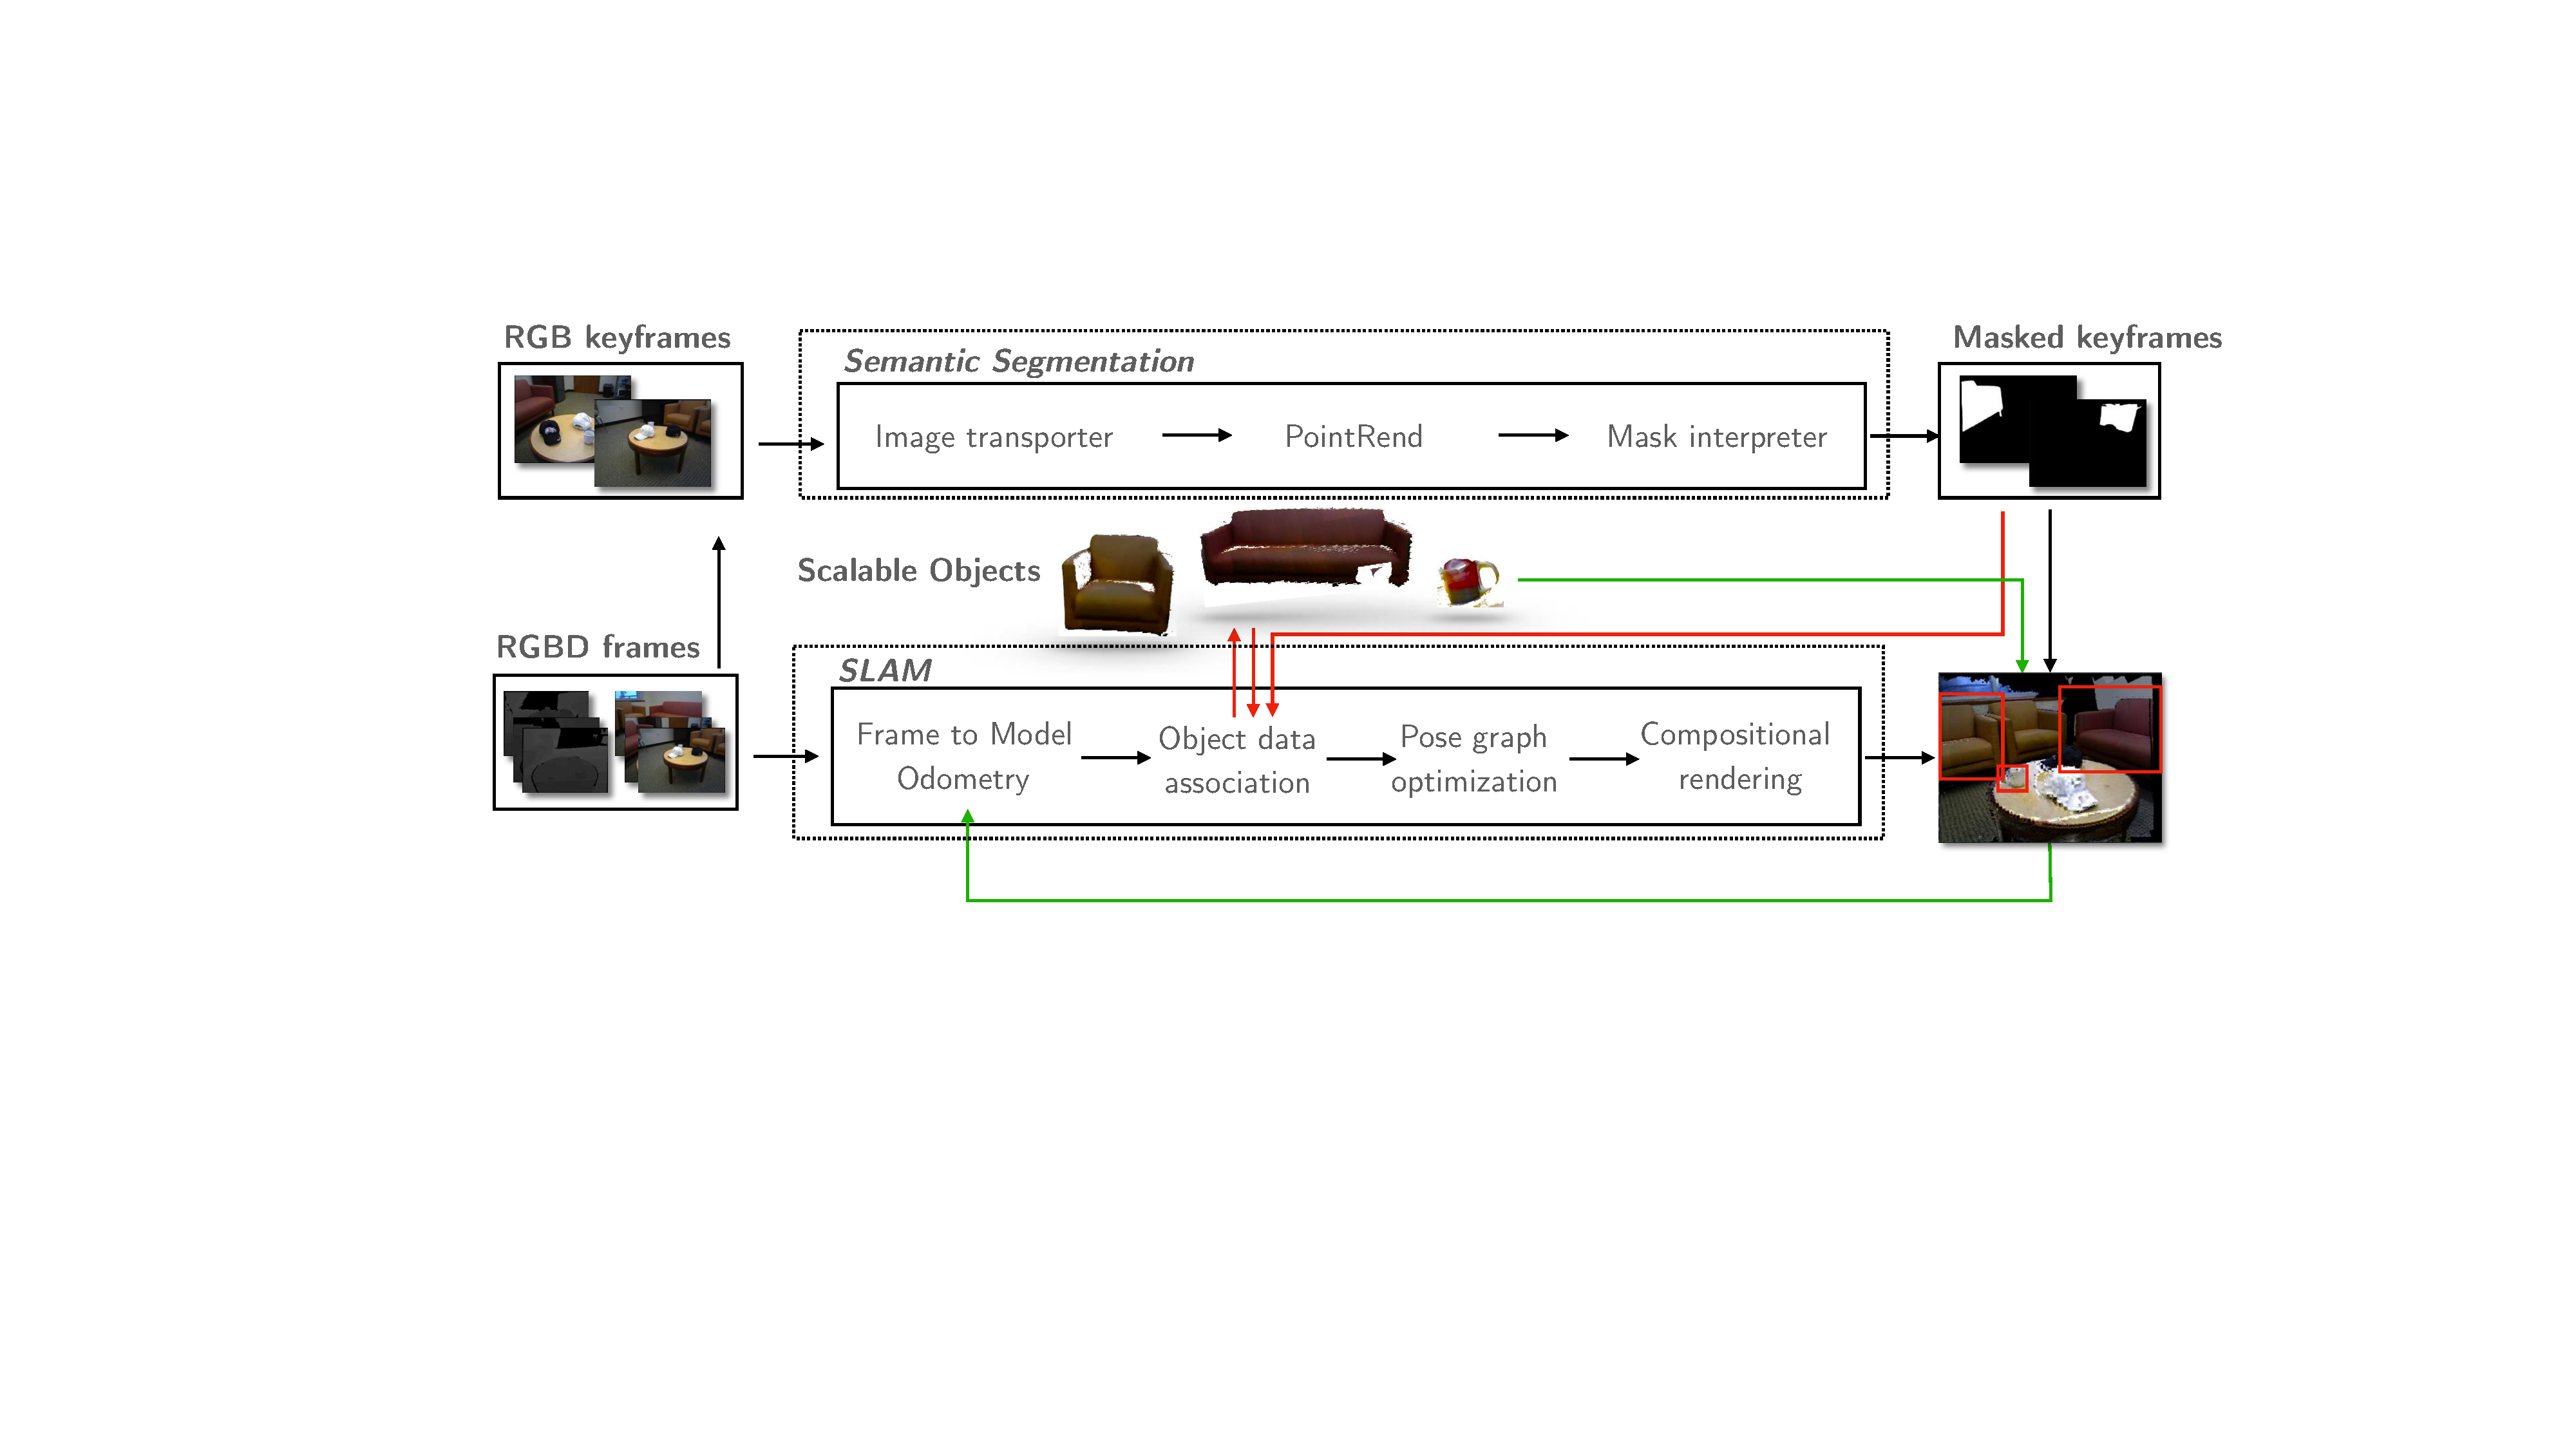
\includegraphics[width=0.90\linewidth]{figs/icra2021-compressed.pdf}
    \caption{\label{fig:overview} System overview: Top shows the deep object segmentation pipeline that runs asynchronously, Masked keyframes from the segmentation pipeline are used in Data association and map update (shown with red lines). Bottom shows the major stages of the reconstruction system, specifically object models are used in tracking via compositional raycasting (shown with green lines).}
    \vspace*{-1em}
 \end{figure*}
